\documentclass[10pt,a4paper]{article}

\bibliographystyle{ieeetr}

\usepackage[margin=1in]{geometry}
\usepackage{graphicx}
\usepackage{subfig}
\usepackage{amsmath}
\usepackage{url}
\usepackage{pgfgantt}
\usepackage{pdfpages}
\usepackage[title]{appendix}

\graphicspath{{./figs/}}

\newcommand{\code}[1]{\texttt{#1}}

\title{A modular kernel for the Raspberry Pi: Progress Report}

\begin{document}

\maketitle

\begin{center}
    Thomas Archbold \\
    1602581 \\
    University of Warwick \\
\end{center}

\section*{Introduction}
% problem that project addresses, motivations (importance of undertaking)
% make sure objectives are clear and clarify why it is a significant undertaking
% and of suitable level for third year project in computer science
While the personal computer has been widely available to the general public for
some time now, the introduction of the Raspberry Pi - a cheap but otherwise
fully capable computer - has made experimenting with computers much more
accessible, and invites tinkering at all levels. Be it simply getting experience
in a new operating system, or interacting with GPIO pins to turn LEDs on and
off, the Pi provides a simple platform for this to take place. There are a
handful of official operating systems available for the Pi \cite{OSes},
addressing issues such as ease-of-installation, Internet of Things integration,
or classroom management, but there is little in the way of experimenting with the
operating system itself. This project attempts to address this gap by providing
customisation of the lowest level software that manages the computer, so that
different options can be explored and their impact can be felt, rather than
dictated. By its end it will provide an operating system for the Raspberry Pi 2
Model B, whose approaches to CPU scheduling, inter-process communication, and
filesystems may be altered by selecting different options at compilation time.

\section*{Background \& Motivation}
% all research I have put into it until this point - good understanding of
% background and how it fits into landscape (does not exist in isolation, before
% or after conception)
% indication of how background information was gained - a few citations that
% have been key sources for project
An operating system is a piece of software which draws together a wide range of
aspects within the field of computer science, from applying knowledge about a
computer's organisation and architecture, to implementing efficient algorithms
on specifically crafted data structures, from resource allocation graphs to
filesystem trees. As such, it should successfully marry much of the theory
behind computer science with its application, to produce software encompassing
the entire field. Thus the main motivation behind the project was to not only
gain experience in systems programming and in interacting with real-world
hardware, but also to draw on these areas of computer science to create one
useful, entirely self-contained piece of software. This is with the goal in mind
that by its end, the project will produce an operating system that offers
configuration to the most fundamental degree, and which can serve as a solid
foundation on which more useful features of modern operating systems can be
added.

Inspiration has been drawn from a number of sources, not only for the project's
conception, but also in guiding some early design decisions. In particular,
Cambridge's \textit{Baking Pi} \cite{BakingPi}, Stanford's \textit{Pintos}
\cite{Pintos}, and \cite{jsandler} have so far been helpful in providing
guidance to achieving a basic functioning operating system, albeit it need of
translating for the Raspberry Pi 2. Some guidance from \cite{littleosbook} has
also been taken, and its use is likely to increase. As for technical references,
the BCM2835/6 Peripherals Manual \cite{BCM2835, BCM2836}, Cortex-A7 MPCore
Technical Reference Manual \cite{TRM}, and ARM Cortex-A Series Programmer's
Guide \cite{PG} have all been useful in finding specific information about the
hardware and how to interact with it on the Pi. The official Github
repositories, in particular \cite{PiDocumentation}, have also helped in this
regard.

\section*{Current progress}
The project is currently at a point at which the operating system is able to
successfully boot in the emulated environment provided by QEMU, determine how
much memory is available, and allocate this dynamically with an interface
similar to \code{malloc()} and \code{free()}. It also boots on real hardware,
but has issues outputting to real HDMI, and the project is currently at a point
where the mailbox peripheral and framebuffer code is being debugged in order to
solve this. Details of what has been achieved for each sub-task is given below.

\subsection*{Development environment}
The project is being developed on a machine running Linux kernel version 4.16
onwards. Since the target environment, the Raspberry Pi 2 Model B, is different
to that on which the project is being developed, a cross-compiler is required to
compile code that will run on the target machine.  Available for download on the
ARM developer website \cite{GNUtoolchain} is the GNU Embedded Toolchain, which
provides tools to target ARM Cortex family of processors, including the GNU
Compiler Collection (GCC). Conveniently this suite of tools is available from
Arch Linux's package manager, Pacman \cite{pacman}, and this is the version of
the cross-compiler being used.

Before writing any code, research had to be undertaken in order to get
acquainted with the low-level development environment, due to little prior
experience in systems programming. This involved skimming over the various
peripherals manuals, technical reference manuals, and programmer's guides for
programming on the Raspberry Pi to learn more about its hardware and how to
interface with it using ARM assembly. \cite{BCM2835} and \cite{BCM2836} detail
the peripherals on board the Raspberry Pi 2 Model B, the layout of their related
registers, and how to read and write them to do meaningful things with the
hardware, while \cite{TRM} and \cite{PG} provided help on ARM assembly's syntax,
and how and when to use specific instructions.

Particularly important so far have been the sections of the peripherals manual
on GPIO and UART, as until the implementation for the mailbox interface is
working, all input and output is done through the serial connection provided by
the UART.  Since there were issues with getting the Pi to run on real hardware,
information about the GPIO peripheral was needed in order to write basic
low-level debugging functions, mainly in the form of getting the green ACT LED
to blink at different points in the program.

\subsection*{boot.s}
The first piece of code written was \code{boot.s}, and is responsible for
providing the basic setup of the entire system, including initialising a minimum
C environment. In particular, it sends three of the four cores on the CPU to
shutdown (to decrease overall complexity of the system, as discussed in the
specification), initialises the stack pointer at address \code{0x8000}, sets up
the BSS segment (where statically-allocated variables that are not explicitly
initialised are stored) and zeroes it out (as required by the C standard), and
then loads our C kernel entry point, \code{kernel\_main}, into memory to begin
its execution. The Program Counter for the kernel starts at address
\code{0x8000} and grows upwards, so the stack can safely start at \code{0x8000}
without interfering with the kernel (as it grows downwards).

\subsection*{linker.ld}
The code in \code{linker.ld} is responsible for linking all of the compiled
object files into one final executable. There are scripts which do this for
user-space programs, but since being the kernel we are our own user-space, we
have to create one for ourselves. The sections that the script defines are as
follows:
\begin{itemize}
    \itemsep0em
    \item \code{.text} - contains executable code
    \item \code{.rodata} - read-only data i.e. global constants
    \item \code{.data} - global variables initialised at compile-time
    \item \code{.bss} - uninitialised global variables
\end{itemize}

We also define the entry point of our entire operating system in this script,
namely the \code{\_start} routine from \code{boot.s}, and also set the symbols
\code{\_\_start} and \code{\_\_text\_start} to be at \code{0x8000}, which is
where the bootloader will put the kernel image. The code from \code{boot.s} will
be put in the first part of this section, \code{.text.boot}. \code{KEEP} tells
the compiler to not try to optimise the code in \code{.text.boot}, and the page
size is set to 4KiB using \code{ALIGN}. The \code{.rodata}, \code{.data}, and
\code{.bss} sections are then declared in similar ways.

\subsection*{Makefile}
The makefile was written to speed up the build process, and there are only a few
features to note. First is that here we specify that we are using the
\code{arm-none-eabi} toolchain, for the compiler to target the Raspberry Pi's
architecture as opposed to our own, in particular the Cortex-A7 processor. The
\code{-fpic} compilation flag is currently being used to generate
position-independent code, to prevent separate applications from interfering
with one another within the single address space while virtual memory is not
implemented. The \code{-ffreestanding} and \code{-nostdlib} flag specify that we
are writing code in a freestanding environment, and as such do not expect much
of the C standard library to exist, and for program startup to not necessarily
to be at \code{main()}.  Specifically, we only have access to the following
header files: \code{<float.h>}, \code{<iso646.h>}, \code{<limits.h>},
\code{<stdalign.h>}, \code{<stdarg.h>}, \code{<stdbool.h>}, \code{<stddef.h>},
\code{<stdint.h>}, and \code{<stdnoreturn.h>}. The rest of the standard library
must be implemented ourselves.

\subsection*{Atags}
The first piece of setup to be done was determining the amount of memory
available to the system. On the Raspberry Pi, the bootloader creates creates a
list of information about the hardware called Atags, places it at address
\code{0x100}, and passes it as the third parameter to \code{kernel\_main} in
register 2. Each tag in the list contains a header consisting of two unsigned
32-bit values: the size of the tag (in 32-bit words), and the tag value. Each
header is then followed by information specific to that tag. To access the
information in each of the tags when we come across them, the layout of each of
the tags \cite{atags} was matched by defining appropriate C structures in
\code{atag.h}.

To find the amount of memory on the device, we skip through the Atags list
(using pointer arithmetic and information about the tag's size in its header)
until we come across the \code{ATAG\_MEM} tag. The function
\code{get\_total\_mem()} then simply returns the value of the \code{size} field
of the \code{atag\_mem} struct.

\subsection*{Organising memory}
The project imposes order on the memory available by splitting it up into 4KiB
pages. To organise the pages, each has been given a header containing
information about whether the it has been allocated, whether it is a kernel
page, and whether this page is part of the heap (used later when dynamically
allocating memory). The headers have been organised into a linked list directly
after the end of the kernel image, using the \code{\_\_end} variable from the
linker script. Each page also stores the virtual address to which it maps; as
virtual memory has not yet been implemented, all pages are simply identity
mapped. The pages are then iterated over and their headers initialised, and each
is added to a linked list of free pages.

Next, page allocation and deallocation was implemented. Allocating a page is
done by simply popping the head of the free page list, setting the appropriate
flags, and returning the address of the page. Freeing, meanwhile, is done by
passing the address of the page to free, again setting the appropriate flags,
and appending this page back to the free page list.

\subsection*{Allocating memory}
A 1MiB portion of memory located directly after the page headers is reserved for
the heap. The struct \code{heap\_segment} is defined for keeping track of heap
allocations, such as the segment size and whether it has been allocated (useful
for avoiding external fragmentation later), and the heap is initialised by
declaring a single heap segment whose size is equal to that of the heap - as
more memory is allocated, this segment will be split into smaller ones, which
may be split further to satisfy requests for differing amounts of memory.

Segment allocation is done by iterating over segments in the heap and finding
the one best satisfying the number of bytes requested, and which is not in use.
If one is found, the address directly after the segment's header is returned.
To free an allocation, we set the appropriate flags, and then attempt to merge
consecutive free segments, checking both to the left and the right of the
current segment.

\subsection*{Serial output}
Initial output was done using the UART on board the Pi, meaning text was sent
and received through serial ports. This was mainly due to simplicity in early
builds of the system, but output in the final version will be done through HDMI,
which requires interfacing with the Mailbox peripheral (discussed later). This
was all done by interacting with the GPIO pins on the Pi, which is done entirely
through Memory Mapped I/O (MMIO) - that is, by reading from and writing to
predefined memory addresses. 

A peripheral on the Raspberry Pi is simply an address to and from which you may
read and write data, and all may be described by an offset from the Peripheral
Base Address; this is \code{0x3f200000} on the Raspberry Pi 2 Model B. Moreover,
a register is a 32-bit chunk of memory that a peripheral may read from or write
to. The BCM2835 Peripherals Manual gives the UART base address as
\code{0x7e201000}\footnote{From the manual: ``Physical addresses range from
\code{0x20000000} to \code{0x20ffffff} for peripherals. The bus addresses for
peripherals are set up to map onto the peripheral bus address range starting at
\code{0x7e000000}. Thus a peripheral listed at \code{0x7ennnnnn} will be
available at physical address \code{0x20nnnnnn}."}. Thus, in \code{gpio.c}, a
serial \code{putc()} is implemented by checking that the FIFO is not full and
writing our data to the Data Register, and \code{getc()} by checking that the
FIFO is non-empty and reading from it.

\subsection*{HDMI output}
The final version, however, will send output through the HDMI port on the Pi. To
do so, the Mailbox peripheral has been used. The Mailbox is a peripheral that
facilitates communication between the ARM CPU and the VideoCore GPU
\cite{Mailboxes}, and starts at offset \code{0xb880}. We may get data from the
GPU via the read register, pass data to the GPU using the write register, and
check if either of these are empty or full using the status register, at offsets
\code{0x00}, \code{0x20}, and \code{0x18} respectively. Furthermore, a channel
is a number that gives meaning to the data being sent to and received from the
GPU - for interacting with HDMI, we need the Property channel, channel 8. This
provides a means to get and set data about various hardware devices, one of
which is the framebuffer.

In order to ask the GPU for a framebuffer, we communicate with it by sending
messages and parsing the received response. The messages sent set the
framebuffer's physical and virtual dimensions, and its colour depth (bits per
pixel). Once all the parameters are set, we ask the GPU for a framebuffer, using
the \code{FB\_ALLOCATE\_BUFFER} tag (defined in \code{mailbox.h} as
\code{0x00040001}). The returned values are a pointer to this framebuffer and
its size. 

\subsection*{Booting on real hardware}
This is the first point at which the project has required testing on real
hardware, in order to verify that a framebuffer is being correctly requested and
supplied by the GPU. This required the kernel to be installed on an SD card and
for it to be run on the physical board of the Pi. It is now helpful to detail
the unique boot process of Pi, which makes this process much easier.

\subsubsection*{The boot process of the Raspberry Pi}
The boot process relies on closed-source proprietary code programmed into the
System on Chip (SoC) processor \cite{Firmware} which cannot be modified.
Importantly, the ARM CPU is not the main CPU, but a coprocessor to the VideoCore
GPU. Upon powerup, the ARM CPU is halted and the GPU is run. The firmware then
loads the bootloader from ROM to the L2 cache and executes it.  This first stage
bootloader mounts the FAT32 boot partition on the SD card so that the second
stage bootloader may be loaded. The first stage bootloader is programmed into
the SoC itself during manufacture and cannot be reprogrammed by the user.  Next,
the second stage bootloader (\code{bootcode.bin}) retrieves the GPU firmware
from the SD card and starts the GPU. The GPU firmware (\code{start.elf}) is
loaded, and allows the GPU to start up the CPU. An additional file
\code{fixup.dat} is used to configure the SDRAM partition between the GPU and
CPU.  Here the kernel image is loaded, the CPU is released from reset, and
control is transferred to it to execute the kernel.

After the operating system is loaded, the CPU runs its own simple operating
system, called Video Core Operating System (VCOS). The kernel can then use this
to communicate with the services it provides (e.g. providing a framebuffer)
using the Mailbox Peripheral and interrupts (the GPU is able to produce ARM
interrupts). The GPU is not only in charge of graphical functions, and also
controls clocks and audio, for example. In this way the GPU firmware is similar
to a normal PC's BIOS (Basic Input/Output System) \cite{Boot1, Boot2}.

\subsubsection*{Loading using Raspbian}
To install the project's kernel onto an SD card, it was copied to an SD card
already containing an operating system, in this case Raspbian \cite{Raspbian},
and its \code{kernel7.img} was replaced with that produced by the Makefile. Now,
when the bootloader would look to load Raspbian's kernel image, it loads the
project's instead.

\subsubsection*{Debugging on real hardware}
On the first attempt, printing via HDMI did not work, despite functioning in
QEMU's simulated environment. In particular, the "rainbow screen" is shown,
signifying that the framebuffer is not being initialised properly. In an attempt
to debug this, assembly code was written, under the guidance of \cite{BakingPi},
to make the green ACT LED blink at certain points in the code, to verify that
these points were being reached successfully. This is the current point at which
the project is in terms of progress.

\section*{Project management}
\subsection*{Development}
The project has been developed incrementally - this has involved deciding on the
next feature to implement, breaking it down into its own set of requirements,
and tackling each of these in turn. An example of this is memory management, for
which it was broken down into getting information about memory through the
Atags, implementing paging, then implementing segmentation and a dynamic memory
allocator. Up to this point in the project there has been little flexibility
in the order in which things are completed, as some of the systems are still
being implemented to even allow ``higher-level'' features to exist. An example of
this is getting the project to work on real hardware before interrupts and
interrupts before scheduling: the former because of QEMU's lack of simulation of a
system timer, and the latter because processes cannot be interrupted if there is
no way to interrupt anything. Once the base systems are implemented, development
can open up more, with more flexibility as to deciding on which features to
develop next. This will of course need to be managed to ensure all areas that
the project aims to address are getting attention.

Version control has been a constant focus during development, and has been
important. Due to the size of this project already, with the amount of code from
a number of different files all contributing to the system's functionality, any
time a change is made that has broken the project where a previous version has
worked has been much less of an issue. In particular, using Git has allowed for
specific differences between commits to be presented clearly, helping to track
down the source of various problems much more quickly.

Progress has been kept in mind by timetabling fortnightly meetings with the
project supervisor. This has allowed progress to be regularly considered, when
otherwise it may be easy to forget about the project in favour of other modules.
Regularly discussing the project has also consolidated things learned over the
course of the fortnight, and help identify exactly what progress has been made.

\subsection*{Testing}
% How have I managed the project so far - may use formal methodology (e.g.
% management of code versions), and can refer to less formal ways of keeping on
% track, e.g. regular meetings with supervisor
As the focus of the project so far has been to set up the foundations upon which
more meaningful work can later on be built, testing has been done entirely
manually, simply as there does not exist the platform to do otherwise at this
stage. In particular, nothing much more can be done when testing if the project
will boot on a physical system other than loading it onto an SD card and
trying it. One aspect that has been able to be checked by unit-testing are
implementations of functions in the C standard library. In this case, for
example when testing \code{printf()}, the function was called with a range of
different values, for example very large, negative, and zero, to test that such
different cases could be handled, and if not, it was then explored manually why
not. In this way, testing has been a slow process, but equally in a way that
demands the necessary attention to detail to be paid to writing a stable
operating system.

\subsection*{Ethical consent}
% state that I have considered it, but not needed
All software being used to develop the project is available under the GNU Public
License. At points in the project's development, informal feedback may be
requested from friends and colleagues for more of the non-functional
requirements, such as usability or how the project is presented. Due to the
informal nature of this feedback, however, any associated ethical, social, or
professional issues are insignificant.

\section*{Progress issues}
\subsection*{Comparison with original timetable}
Progress has largely been in line with that which was originally scheduled.
Early on, progress was even slightly ahead of the timetable, particularly when
writing \code{boot.s} and \code{linker.ld}, but this is largely due to there
being little need to stray from the example code provided by \cite{OSDevBoot}.
Overall, what was achieved compared to what was timetabled differed little in
the first five weeks of the project. It was attempting to move to working and
testing on real hardware where the two began to diverge - although it could boot
on real hardware (evidenced by flashing the ACT at different times), problems
arose when printing output to a real HDMI screen. Due to the limited facility to
debug at this level, it has been particularly difficult to work towards a
solution to this problem, and the project has fallen behind by a few weeks on
this goal. As a result of this, at the time of writing, progress should be
underway on loading programs into memory for execution, whereas in reality
processes have not even begun development yet. Interrupts and processes should
also have been completed by this point, and while progress has started on the
former, the system will need to operate on real hardware for them to be finished,
due to QEMU's lack of system timer. Therefore, interrupts and processes will not
be able to be completed until the issue of outputting to HDMI is resolved.

A reason for this oversight in the timetable is related to underestimating the
problems that could arise in the transition from an emulated environment to a
fully real one, as well as the time required to fix them. Furthermore, while
course load was considered when writing the initial schedule, unforeseen issues
with other pieces of coursework have interfered with progress on this project,
more than previously accounted for. Time was however set aside during the winter
holidays specifically to catch up in the case of delays, and as such the revised
timetable, given in Appendix A, only differs slightly at the start of Term 2.

\subsection*{Areas for timetable revision}
The first change made to the timetable is the addition of several tasks, and
merging of others into one. For example, booting has been given its own section,
and memory management has been broken into organising memory by accessing Atags,
and dynamic memory allocation. HDMI support has also been split into sections on
mailboxes, framebuffers, and HDMI output as the task to get them working was
larger than previously thought and deserving of more separate goals. Booting on
real hardware has been added as a section to signify the time spent debugging
the problems with transitioning on the real device, and is currently active.

Virtual memory has been introduced, and where previously filesystems was split
into persistent and load-on-request, it is now one block. Userspace is now a
larger section, and encompasses the fork and execute and threading goals. The
shell section has been extended to highlight its ongoing nature, while the
stretch goals of networking and a ext editor have been added in similarly
extended blocks of time, as it is unlikely they will be completely done before
the project's end.

One section that has been dropped entirely from the timetable is the development
of a C standard library. That is not to say that it is not being implemented,
but that it is only an auxiliary task - it will be continually developed as
needed by other parts of the operating system, and not, as previously it might
have implied, for its own sake. As an example, \code{itoa()} and \code{printf()}
have been implemented, not because they show up in Linux, but because they
provide meaningful functionality for tasks such as debugging. Therefore, this
section is still present, albeit implicitly, as it is so closely tied to all
other tasks.

Further, tasks have been shifted around in the revised timetable compared to the
original. Firstly, up to 25 November, 2018, the timetable now reflects the
actual progress which was made, showing that booting and displaying on real
hardware is still in progress, and interrupts will be started this week.  Most
of the tasks following this in the original timetable have been pushed back to
highlight this delay. Scheduling now carries into Term 2, and scheduled time to
implement more schedulers has also been moved forward where previously it was to
be started later. Filesystems have also been moved earlier in the term, as has
message passing. This is to allow enough time for  compilation configuration to
be developed, which has also been moved forward, to allow enough time to get it
working well for the presentation. The endpoint for the presentation has also
moved forwards to reflect the true deadline, while work on the final report will
also now start much earlier.

% overview of work so far, including
%   technical content - what work have I done, meaningful summary of significant
%   aspects
%   progress - review progress against timetable. If unexpected delays, how have
%   they been dealt with?

\section*{Next steps}
% outline plans for next term and any alterations to original ideas
% updated timetable with as much detail as possible
For the rest of Term 1, most efforts will be dedicated to debugging the issue
with printing on HDMI on real hardware. The nature of the problem makes the
process more difficult in that debugging will rely solely on tweaking the flash
of an LED. This issue should find resolution during the holidays. Furthermore,
to make up the deficit in progress caused by this delay, more attention will
need to be paid towards interrupts, exceptions, and processes, in order to
finish them in a timely manner so that work can be at least started on
scheduling, inter-process communication, and synchronisation before the calendar
year's end.

Some further research will also need to be undertaken before the start of Term 2
to decide on a filesystem to implement, and assess whether to implement custom
one or one that is already established, such as SFS, FAT, BMFS, or something
else still \cite{Filesystems}. At this point, there is little to distinguish the
project from any other hobbyist operating system, given that there is nothing it
does that is special or particularly unique at this stage. Over next term is
where the project will begin to diverge from other operating systems and take on
its own form, that is, in granting the user a degree of customisation at a low
level which others do not provide. Going into the start of Term 2, focus will be
on developing the features that will begin to differentiate this operating
system from others, namely different approaches to CPU scheduling and
inter-process communication, and thought will need to be put into the
interface for customising the operating system at compile-time early, to ensure
a working solution by the time of the presentation.

\section*{Reflection}
% reflection and appraisal - assessment on how things have gone so far. Any
% lessons learned to make future progress smoother?
The progress made with the project so far has been pleasing; having little
experience in systems programming prior to starting this project, it has been
fulfilling learning about every aspect of the Raspberry Pi in minute detail,
which is indeed required to make things work at this low-level. While it has been
noted that at this point there is little to distinguish this piece of work from
any other hobbyist operating system, it is nonetheless satisfying to have set
this ground work which is still, all things considered, a custom operating
system that is capable of running on a Raspberry Pi. Furthermore, despite the
issue caused by the framebuffer, it has been a fun challenge to develop a
debugging solution for this, and while a blinking green LED may not be a core
feature of the final project, learning how to use the GPIO and doing so in
assembly has been another valuable learning experience. Overall, despite the
setbacks caused by running on real hardware, the project is progressing well,
and while difficulty is expected to pick up into next term, so too is time spent
working on it, hopefully allowing for a smooth transition in between terms and
for steady progress to continue being made.

\bibliography{bibliography}

\begin{appendices}

    \pagenumbering{gobble}

    % Revised Timetable
    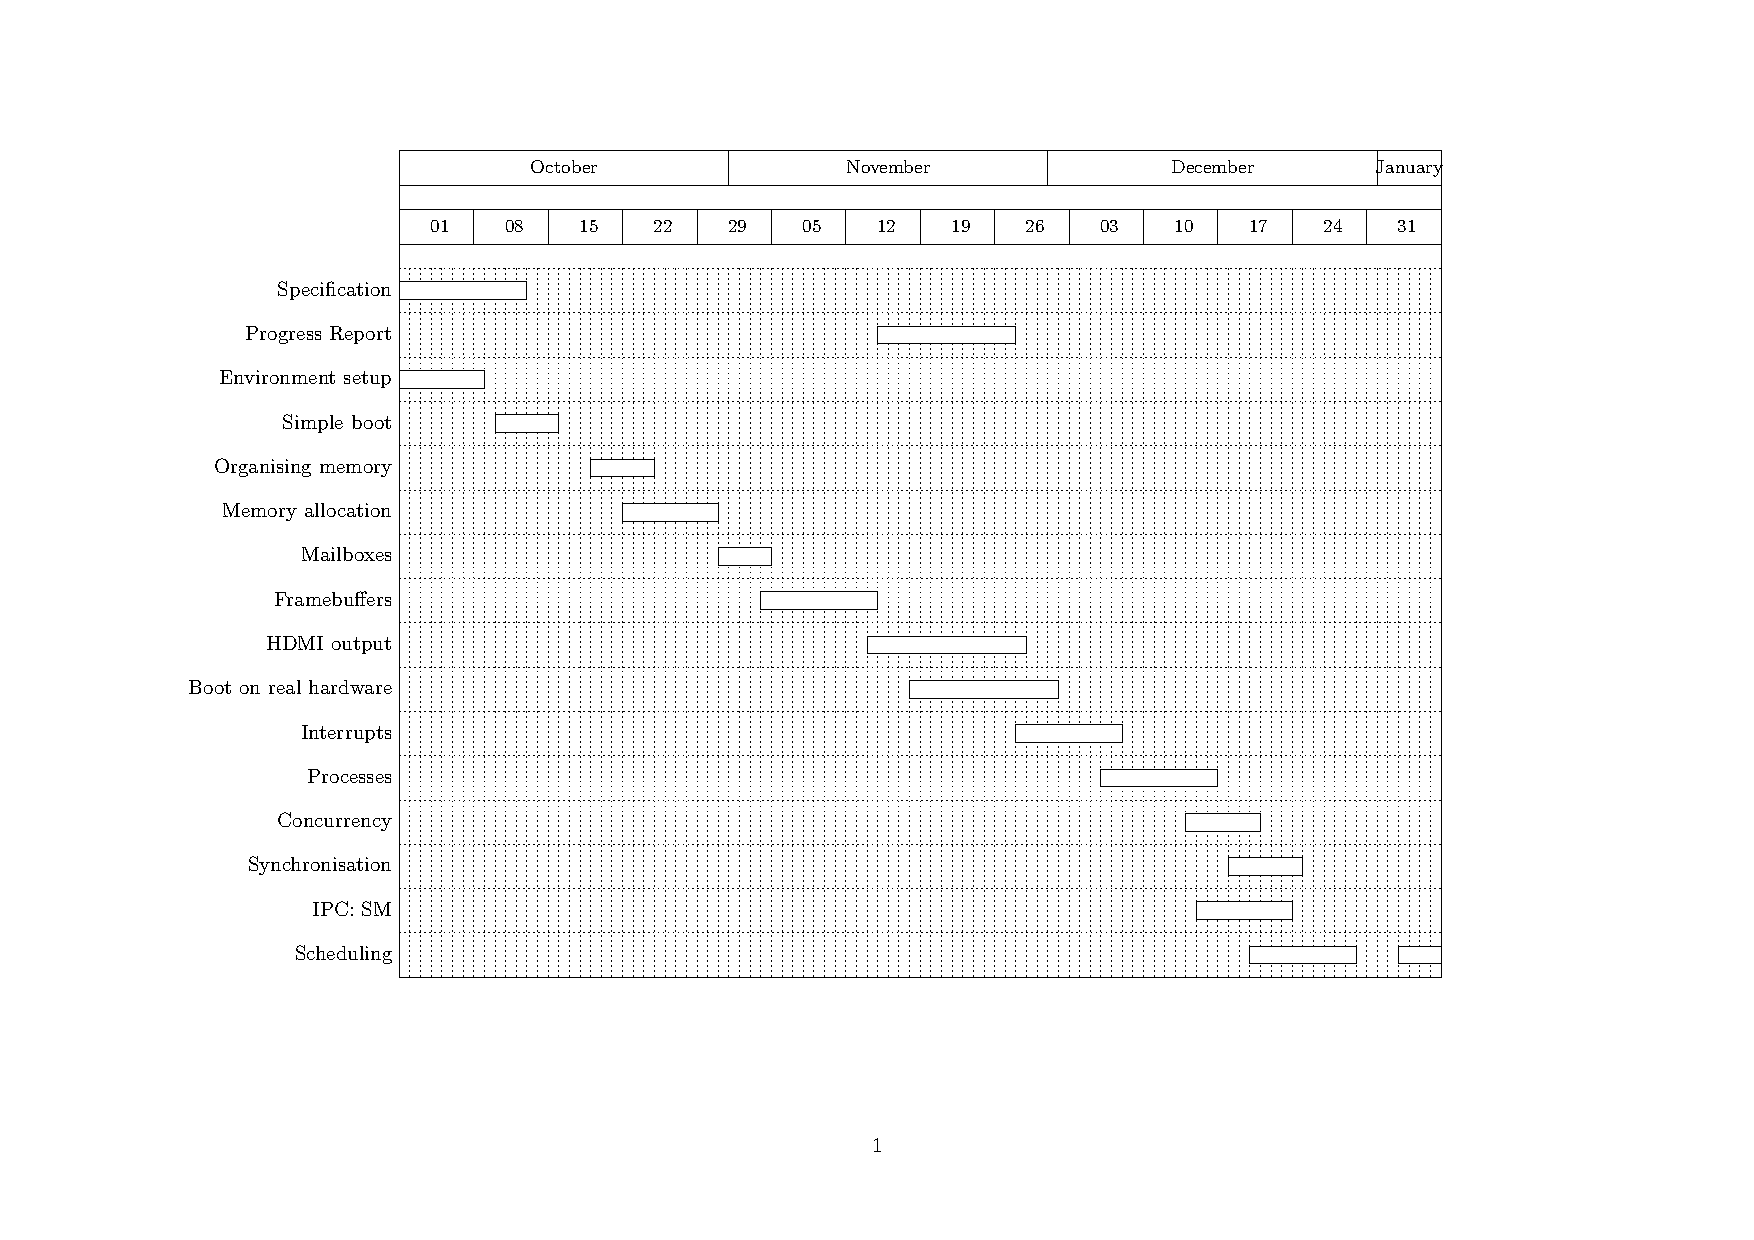
\includepdf[landscape=true,pages=1,pagecommand={\section{Revised Timetable}}]{timetable/timetable.pdf}
    \includepdf[landscape=true,pages=2,pagecommand={}]{timetable/timetable.pdf}

    % Project Specification
    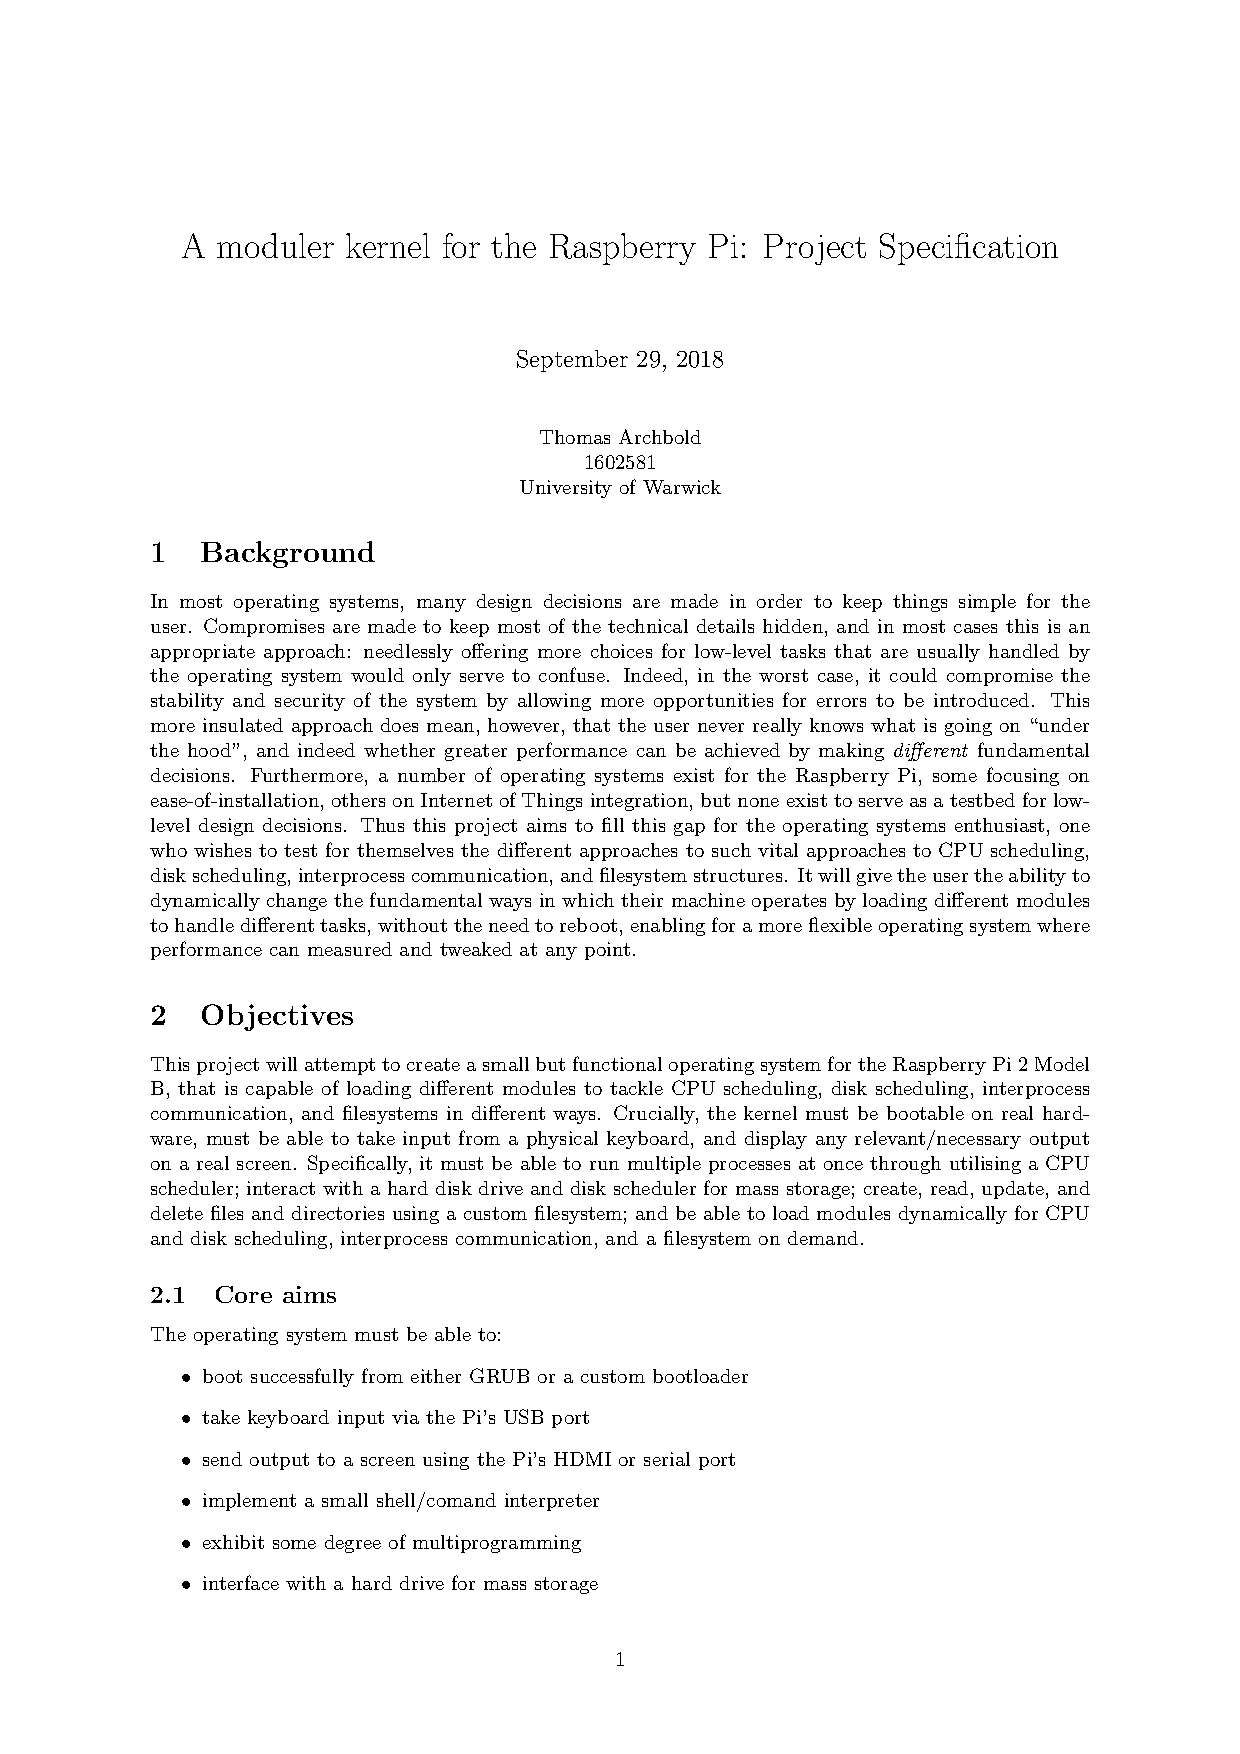
\includepdf[pages=1,pagecommand={\section{Project Specification}}]{../specification/specification.pdf}
    \includepdf[pages=2-6,pagecommand={}]{../specification/specification.pdf}
    \includepdf[landscape=true,pages=7-,pagecommand={}]{../specification/specification.pdf}

\end{appendices}

\end{document}
